\documentclass[a4paper, 14pt]{extreport}
\pagestyle{plain}

\usepackage[T1, T2A]{fontenc}	
\usepackage[english,russian]{babel} %Русские шрифты
\usepackage[utf8]{inputenc}

\usepackage{extsizes} % вроде бы для размера шрифтов

\usepackage{graphicx} % для вставки картинок
\usepackage{amssymb,amsfonts,amsmath,amsthm,mathrsfs} % математические дополнения от АМС
\usepackage{hyperref} %для гиперссылок
\usepackage{indentfirst} %отступ для первой главы параграфа
\usepackage{upgreek} %для красивенькой буквы фи
\usepackage{listings} % для листинга кода
\usepackage{color} % для использоания цветного фона в листинге кода
\usepackage[justification=centering]{caption}  % для центрирования подписи в картинке
\usepackage{subcaption}
\usepackage{tocloft} % для нормального размера названия заголовка содержания
\usepackage{caption} % для человеческих подписей к рисункам
\usepackage{titlesec}
\usepackage[style=russian]{csquotes} % угловые кавычки
\usepackage{float} % для нормального позиционирования картинок


\usepackage{geometry} % отступы и все такое
 \geometry{
 a4paper,
 left=30mm,
 right=10mm,
 top=20mm,
 bottom=20mm,
 } 

\unitlength=1mm %Единица измерения длины в рисунках - 1 мм
\renewcommand{\bfdefault}{b}   % Делает жирный шрифт менее широким	
\renewcommand{\Re}{\text {Re}}
\renewcommand{\Im}{\text {Im}}
\renewcommand{\baselinestretch}{1.5} % межстрочный интервал
\setcounter{page}{2} % старт номера страниц
\setcounter{secnumdepth}{3} % нумерация subsubsection
\setcounter{tocdepth}{3} % subsubsection в оглавлении

\makeatletter
\renewcommand\@biblabel[1]{#1.} % нормальная нумерация источником
\makeatother

\setlength{\cftbeforetoctitleskip}{-3em}

\lstset{ %настроки листинга кода. чтобы красивенько было, вот это вот все
	language=Python,
	keepspaces=true,
	numbers=left,
	linewidth=15cm,
	frame=L,
	basicstyle=\footnotesize,
	showstringspaces=false,
	inputencoding=utf8,
	extendedchars=\true
}

%change semicolon to defis in pictures:
\RequirePackage{caption}
\DeclareCaptionLabelSeparator{defffis}{ -- }
\captionsetup{justification=centering, labelsep=defffis}

% отступ в заголовках
\newlength{\normalparindent}
\AtBeginDocument{}
\titleformat{name=\section}[block]
  {\Large\bfseries}
  {\hspace{\normalparindent}\thesection}
  {0.5em}
  {}
	
% отступ в подзаголовках
\titleformat{name=\subsection}[block]
  {\large\bfseries}
  {\hspace{\normalparindent}\thesubsection}
  {0.5em}
  {}
	
% отступ в подподзаголовках	
\titleformat{name=\subsubsection}[block]
	{\bfseries}
	{\hspace{\normalparindent}\thesubsubsection}
  {0.5em}
  {}

% chapters format
\titleformat{\chapter}[display]   
{\normalfont\huge\bfseries\center}
{\chaptertitlename\ \thechapter}
{0pt}
{\huge}   
\titlespacing*{\chapter}{0pt}{-50pt}{0pt}

\AtBeginDocument{
   \let\div\relax % чтобы операторы дивергенции и градиента чуть что красивенько писались
   \DeclareMathOperator{\div}{div}
          \DeclareMathOperator{\grad}{grad}
          \setlength{\normalparindent}{\parindent} % для выравнивания заголовков
}


% шрифты на linux более гладкие
\pdfpkmode{dpdfezzz}
\pdfpkresolution=8000

\begin{document}
\renewcommand{\figurename}{Рисунок} % чтобы рисунки назывались не "Рис.", а "Рисунок", должно быть под Russian, ибо собьется
\renewcommand{\contentsname}{\hfill\Large ОГЛАВЛЕНИЕ \hfill}
\renewcommand{\cftaftertoctitle}{\hfill}


\tableofcontents



\newpage
\phantomsection
\begin{center}
	\Large{\textbf{РЕФЕРАТ}}
\end{center}

Отчет о преддипломной практике, 28 страниц, 16 рисунков, 3 источника, 1 приложение.

\textbf{\textit{Ключевые слова:}} ТЕОРИЯ УПРУГОСТИ, МЕТОД КОНЕЧНЫХ 
ЭЛЕМЕНТОВ, ТЕНЗОР ДЕФОРМАЦИИ, PYTHON, FEniCS, 
GMSH, \\ PARAVIEW

\textbf{\textit{Объект исследования:}} граничная задача теории 
упругости в области сложной формы.

\textbf{\textit{Цель работы:}} реализовать метод приближенного решения
задачи теории упругости в рассматриваемой области с помощью пакета
\texttt{FEniCS} и проанализировать результаты.

\textbf{\textit{Методы исследования:}} метод конечных элементов.

\textbf{\textit{Результат:}} сценарий на языке \texttt{Python},
использующий возможности пакета \texttt{FEniCS}.

\textbf{\textit{Область применения:}} численные решения краевых 
дифференциальных задач эллиптического типа в частных производных.

\begin{center}
	\Large{\textbf{РЭФЕРАТ}}
\end{center}

Даклад ад прэддыпломнаый практыцы, 28 старонак, 16 малюнкаў, 3 крыніцы, 1 дадатак.

\textbf{\textit{Ключавыя словы:}} ТЕОРИЯ ПРУГКАСЦІ, МЕТАД КАНЧАТКОВЫХ \\
ЭЛЕМЕНТАЎ, ТЕНЗАР ДЭФАРМАЦЫІ, PYTHON, FEniCS, 
GMSH, \\
PARAVIEW.

\textbf{\textit{Аб'ект даследавання:}} межавая задача тэорыі 
пругкасці ў вобласці складанай формы.

\textbf{\textit{Мэта работы:}} пабудаваць метад для колькаснага 
рашэння задачы теорыі пругкасці ў расгледжваемай вобласці з
дапамогай пакета \texttt{FEniCS} и прааналізіраваць вынікі.

\textbf{\textit{Метады даследавання:}} метад канчатковых элементаў.

\textbf{\textit{Вынiкi:}} праграмма на мове \texttt{Python},
якая выкарыстае магчамасці пакета \texttt{FEniCS}.

\textbf{\textit{Вобласть выкарыстання:}} колькасныя рашэнні мэжавых 
дыфференцыяльных задач элліптычнага тыпу ў прыватных вытворынх.


\begin{center}
	\Large{\textbf{SUMMARY}}
\end{center}

Externship report, 28 pages, 16 pictures, 3 sources, 1 appendix.

\textbf{\textit{Keywords:}} ELASTICITY THEORY, FINITE ELEMENT METHOD,
STRAIN TENSOR, PYTHON, FEniCS, GMSH, 
PARAVIEW.

\textbf{\textit{Research object:}} boundary problem of the elasticity
theory in complex domain.

\textbf{\textit{Purpose:}} to build a method for numerical solving 
elasticity theory problem in current domain using the \texttt{FEniCS}
package and to analyze the results.

\textbf{\textit{Research methods:}} the finite element method.

\textbf{\textit{Result:}} Python script which use \texttt{FEniCS}
package abilities.

\textbf{\textit{Application field:}} numerical solving of the
boundary problems for partial differential equations of the elliptic type.


\newpage
\phantomsection
\begin{center}
\addcontentsline{toc}{section}{ВВЕДЕНИЕ}
	\Large{\textbf{ВВЕДЕНИЕ}}
\end{center}

Многие процессы в природе приводят к уравнениям в частных производных
эллиптического типа, и, чтобы проанализировать результаты данных процессов,
эти уравнения должны быть решены.

Однако, не все так просто. Зачастую краевые задачи для эллиптических
уравнений невероятно сложно решить аналитически, например, по причине
нетрадиционной формы области, на которой сформулирована задача.
Поэтому, такие задачи нужно решать численными методами.

Метод конечных элементов (\cite{finite_element_method}) -- эффективный метод численного решения краевых задач
эллиптического типа. Он и используется в данной работе.

Первый раздел данной работы посвящен неформальному описанию рассматриваемой
задачи.

Во втором разделе описана формальная постановка задачи.

В третьем разделе рассмотрено все, что касается вычислительного эксперимента:
процессы моделирования области и численного решения задачи, а также 
приведены иллюстрации результатов.


\newpage
\chapter{Постановка задачи}
\section{Формулировка задачи}
\subsection{Общая формулировка задачи теории упругости}


Под влиянием приложенных сил твердые тела могут изменять свои форму и объем, 
т.е. в той или иной степени деформироваться.

Пусть радиус-вектор \, $\textbf{x} = (x_1, x_2, x_3)$ \, описывает координаты 
некоторой материальной точки твердого тела до воздействия на него внешних сил,
а \, $\textbf{x}' = (x'_1, x'_2, x'_3)$ \, -- радиус вектор той же материальной
точки после действия внешних сил. Перемещение точки характеризуется 
\textit{вектором упругих деформаций} \,$\textbf{u} = \textbf{x}' - \textbf{x}$, 
где  $u_i = x'_i - x_i$. Деформированное состояние тела
полностью описывается заданием вектора упругих деформаций для каждой точки тела.

Задача \texttt{теории упругости} (\cite{math_elasticity_theory}) состоит в 
отыскании вектора $\textbf{u}$ как функции, исходя из начальных условий.

\subsection{Краткое описание рассматриваемой задачи}

Будем решать задачу для трехмерной области сложной формы, диаметральное сечение
которой представлено на рисунке \ref{fig: domain}.
\begin{figure}[h]
	\center
	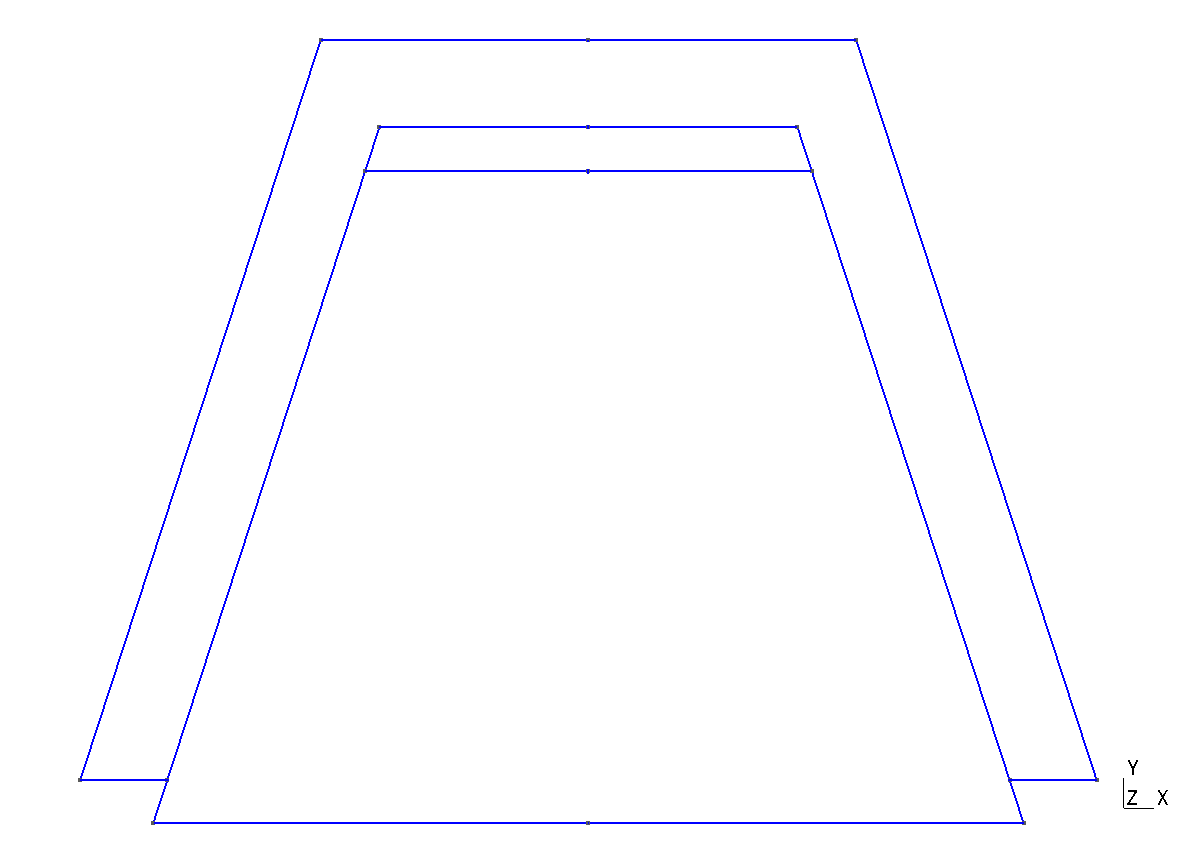
\includegraphics[scale=0.3]{pictures/1.png}
	\caption{Диаметральное сечение области}
	\label{fig: domain}
\end{figure}

Область представляет собой пару усеченных конусов, один из которых
\enquote{надет} на другой. Между конусами имеется свободное пространство.

К верхнему основанию внешнего конуса прикладывается нагрузка $\textbf{g}$
под некоторым углом.

Требуется определить напряженно-деформированное состояние тела после
действия нагрузки.

Такое моделирование в реальной жизни может быть применено к
процессу коронирования зубов, когда коронка (внешний конус) надевается
на сточенный зуб (внутренний конус). Образующие части кумулятивного
элемента состоят из разных материалов, откуда следуют различия в их
физических свойствах. Нужно подобрать правильный материал для коронки
и правильно ее поместить на зуб, чтобы она не ломалась, 
не соскальзывала и пациент был счастлив. Для этого 
проводится моделирование и оценка результатов.


\section{Формальная постановка задачи}
\subsection{ Дифференциальная формулировка}

Рассмотрим на диаметральном сечении основные части нашей области 
(рисунок \ref{fig: marked_domain}).
\begin{figure}[ht]
	\center
	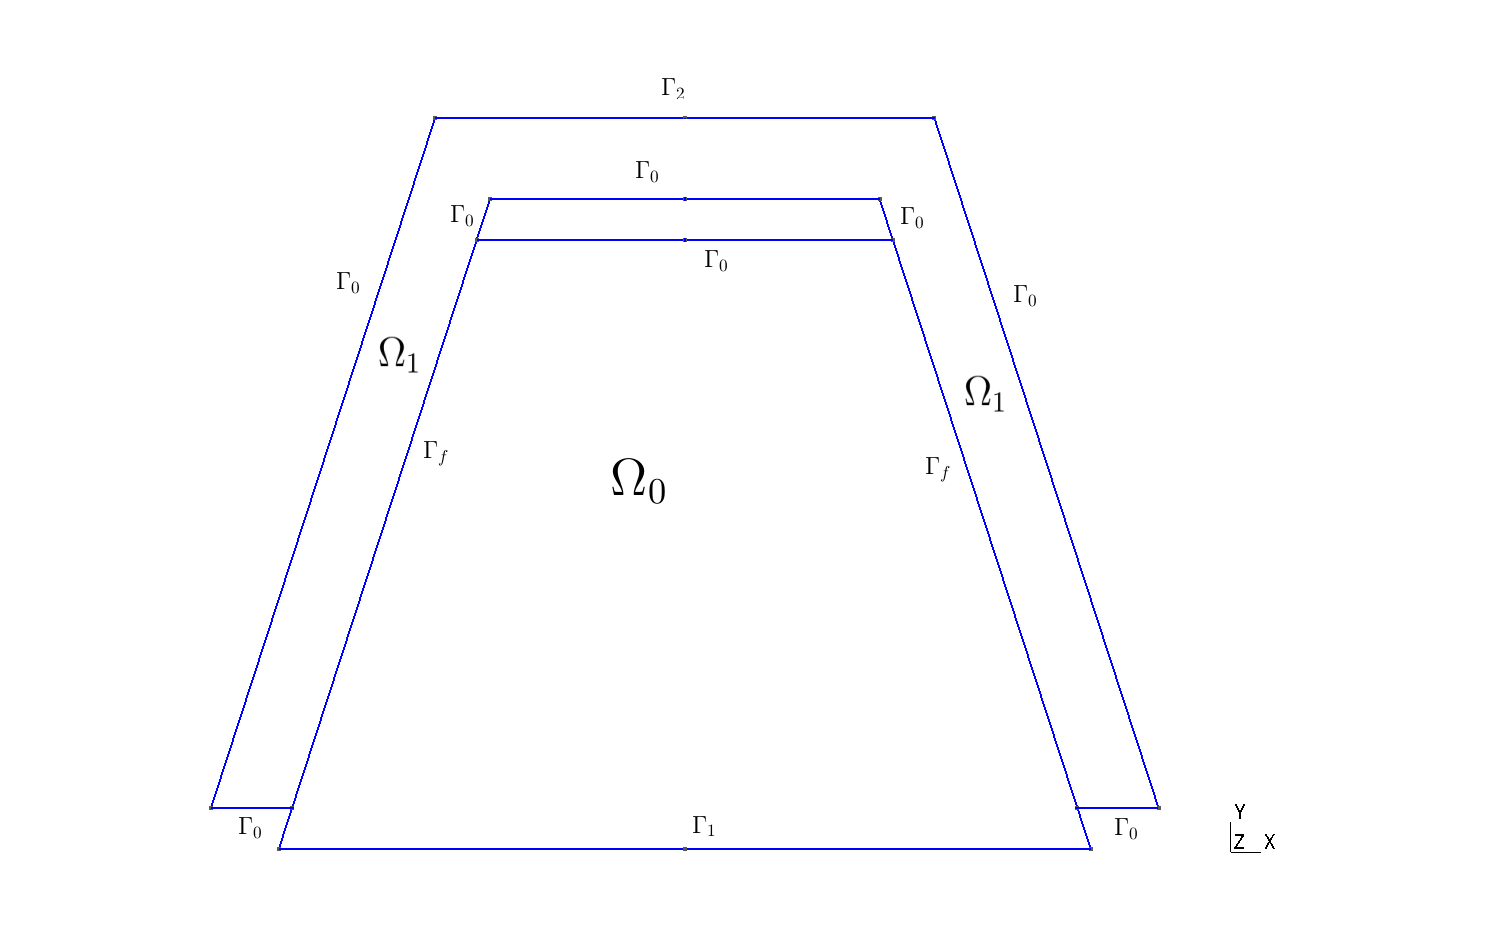
\includegraphics[scale=0.25]{pictures/marked_domain.png}
	\caption{Обозначение составляющих частей области (в разрезе)}
	\label{fig: marked_domain}
\end{figure}

Рассмотрим задачу в следующей дифференциальной формулировке:
\begin{equation}
	\label{eq:1}
	\nabla\!\cdot\!\sigma(\textbf{u}) = \textbf{0}, \textbf{x} \in \Omega = \Omega_0 \cup \Omega_1
\end{equation}
с граничными условиями:
\begin{equation}
	\label{eq: boundary_conditions}
	\begin{aligned}
		(\sigma(\textbf{u}), \textbf{n})(\textbf{x}) 	  	  &= \textbf{0},   &&\textbf{x} \in \Gamma_0,\\
		(\sigma(\textbf{u}), \textbf{n}) 				  	  &= \textbf{g},   &&\textbf{x} \in \Gamma_2, \; \textbf{g} = (g_1, g_2, g_3)\\
		\textbf{u}(\textbf{x})							  	  &= \textbf{0},	   &&\textbf{x} \in \Gamma_1,\\
		(\sigma(\textbf{u}), \textbf{n})\vert_{\Gamma_{f - 0}} &= 
			(\sigma(\textbf{u}), \textbf{n})\vert_{\Gamma_{f + 0}},             &&\textbf{x} \in \Gamma_f,
	\end{aligned}
\end{equation}
где $\sigma(\textbf{u})$  -- \texttt{тензор напряжений}, \textbf{n} -- вектор нормали
к поверхности. 

Граничные условия (\ref{eq: boundary_conditions}) означают, что к части поверхности 
$\Gamma_2$ приложена нагрузка, часть поверхности $\Gamma_1$ жестко закреплена, 
а на части поверхности $\Gamma_f$ выполняются условия сопряжения: напряжения 
с одной стороны поверхности противоположны по направлению напряжениям с 
другой стороны и равны по модулю.

Такая постановка задачи также называется \textit{постановкой в напряжениях}.

Известна связь между тензором напряжений $\sigma(\textbf{u})$ и \texttt{тензором деформаций}
$\varepsilon(\textbf{u}) = \frac{1}{2}(\nabla\textbf{u} + (\nabla\textbf{u}^T))$:
\begin{equation*}
\sigma(\textbf{u}) = \lambda \nabla\!\cdot\!\textbf{u}\textit{I} + 2\mu\varepsilon(\textbf{u})
\end{equation*}
где $\lambda, \mu $ \, - \texttt{коэффициенты Ламе}, характеризующие упругие свойства тела,
\textit{I} - единичный тензор второго ранга.

Отсюда  можно получить формулировку (\ref{eq:1}) в \textit{перемещениях} (в векторной форме):
\begin{equation}
	\label{eq: 2}
	\mu\Delta\textbf{u} + (\lambda + \mu)\grad\!\nabla\!\cdot\!\textbf{u} = \textbf{0}
\end{equation}



\subsection{ Вариационная формулировка}
При построении дискретной задачи для решения ее методом конечных элементов 
используется вариационная формулировка исходной дифференциальной задачи.
Опишем ее.

Введем следующие функциональные пространства:
\begin{itemize}
	\item $V = \{ \textbf{u(\textbf{x})} \in \textbf{H}^1(\Omega) \vert \textbf{u(\textbf{x})} = \textbf{0}, \textbf{x} \in \Gamma_1 \}$ --
	пространство \textit{триальных} функций;
	\item $\hat{V} = \{ \textbf{v(\textbf{x})} \in \textbf{H}^1(\Omega) \vert \textbf{v(\textbf{x})} = \textbf{0}, \textbf{x} \in \partial\Omega \}$ --
	пространство \textit{тестовых} функций.	
\end{itemize}

Для начала, скалярно домножим (\ref{eq:1}) на тестовую функцию $\textbf{v} \in \hat{V}$, 
а затем проинтегрируем по области $\Omega$.

По свойствам оператора дивергенции,
\begin{equation}
	\label{eq: 3}
	\nabla\!\cdot\!(\sigma(\textbf{u}), \textbf{v}) = (\textbf{v}, \nabla\!\cdot\!\sigma(\textbf{u})) +
		(\sigma(\textbf{u}), \nabla\textbf{v})
\end{equation}

Следовательно,
\begin{equation}
	\label{eq: 4}
	0 = \int\limits_\Omega{(\nabla\!\cdot\!\sigma(\textbf{u}), \textbf{v})}d\textbf{x} = 
		\int\limits_\Omega{\nabla\!\cdot\!(\sigma(\textbf{u}), \textbf{v})}d\textbf{x} - 
		\int\limits_\Omega{(\sigma(\textbf{u}), \nabla \textbf{v})}d\textbf{x}
\end{equation}

К первому слагаемому (\ref{eq: 4}) применим формулу Грина:
\begin{equation}
	\label{eq: 5}
	\begin{aligned}
		& \int\limits_\Omega{\nabla\!\cdot\!(\sigma(\textbf{u}), \textbf{v})}d\textbf{x} = 
		\int\limits_{\Omega_0}{\nabla\!\cdot\!(\sigma(\textbf{u}), \textbf{v})}d\textbf{x} \; +  \;
		\int\limits_{\Omega_1}{\nabla\!\cdot\!(\sigma(\textbf{u}), \textbf{v})}d\textbf{x} = \\
		& = \int\limits_{\partial\Omega_0}{((\sigma(\textbf{u}), \textbf{v}), \textbf{n})}dS + 
		\int\limits_{\partial\Omega_1}{((\sigma(\textbf{u}), \textbf{v}), \textbf{n})}dS = \\
		& = \int\limits_{\Gamma_2}{((\sigma(\textbf{u}), \textbf{v}), \textbf{n})}dS + 
		\int\limits_{\Gamma_f}{((\sigma(\textbf{u}), \textbf{n}_0) + (\sigma(\textbf{u}), \textbf{n}_1), \textbf{v})}dS + \\
		& + \int\limits_{\Gamma_0}{((\sigma(\textbf{u}), \textbf{v}), \textbf{n})}dS,
	\end{aligned}
\end{equation}
где $\textbf{n}_0$ и $\textbf{n}_1$ - внешняя и внутренняя нормали к поверхности $\Gamma_f$,
т.е. они направлены в разные стороны, а значит, скалярные произведения с этими элементами 
отличаются лишь знаком, т.е. подынтегральное выражение интеграла по границе $\Gamma_f$ 
равно нулю.

Исходя из последнего утверждения, граничных условий и определения пространства $\hat{V}$,
(\ref{eq: 5}) преобразуется в:
\begin{equation}
	\label{eq: 6}
	\int\limits_\Omega{\nabla\!\cdot\!(\sigma(\textbf{u}), \textbf{v})}d\textbf{x} = 
	\int\limits_{\Gamma_2}{(\textbf{g}, \textbf{v})}dS
\end{equation}

Преобразовав подынтегральное выражение (\ref{eq: 4}) с учетом свойств тензоров, получим:
\begin{equation}
	\label{eq: 7}
	\int\limits_\Omega{(\sigma(\textbf{u}), \nabla \textbf{v})}d\textbf{x} = 
	\int\limits_{\Omega_0}{(\sigma(\textbf{u}), \varepsilon(\textbf{u}))}d\textbf{x} + 
	\int\limits_{\Omega_1}{(\sigma(\textbf{u}), \varepsilon(\textbf{u}))}d\textbf{x}
\end{equation}

В силу (\ref{eq: 6}) и (\ref{eq: 7}), (\ref{eq: 4}) преобразуется в:
\begin{equation}
	\label{eq: 8}
	\int\limits_{\Omega_0}{(\sigma(\textbf{u}), \varepsilon(\textbf{u}))}d\textbf{x} + 
	\int\limits_{\Omega_1}{(\sigma(\textbf{u}), \varepsilon(\textbf{u}))}d\textbf{x} = 
		\int\limits_{\Gamma_2}{(\textbf{g}, \textbf{v})}dS,
\end{equation}
что также можно записать в виде:
\begin{equation}
	\label{eq: 9}
	a(\textbf{u}, \textbf{v}) = L(\textbf{v}),
\end{equation}
где:
\begin{itemize}
	\item $a(\textbf{u}, \textbf{v}) : V \times \hat{V} \rightarrow \mathbb{R}$ \,-- \textit{билинейная форма};
	\item $L(\textbf{v}) : \hat{V} \rightarrow \mathbb{R}$ \, -- \textit{линейная форма}.
\end{itemize}

Задача состоит в том, чтобы отыскать такую  $\textbf{u} \in V$, 
которая удовлетворяет (\ref{eq: 9}).


\chapter{Реализация численного алгоритма}
\section{Построение области и сетки}

Одним из ключевых моментов в данной работе, как и при моделировании 
любой задачи математической физики, является построение области, 
на которой исследуется данная задача.

В данной работе для этой цели использовался free-software
пакет \texttt{Gmsh}. С его помощью можно строить 
области различной формы путем объединения и преобразования
простейших элементов в более сложные (точки в линии, линии в контуры;
контуры задают поверхности, поверхности - объемы), а также генерировать 
сетку.

Для работы с формированием области используется файловый формат 
\texttt{.geo}, для сеток - \texttt{.msh}.
\subsection{Формирование области}
\textbf{Теоретическое моделирование области}

Область, которая была проиллюстрирована на рисунке (\ref{fig: domain}),
можно построить, задав следующие параметры:
\begin{itemize}
	\item height -- высота внутреннего конуса;
	\item width -- радиус нижнего основания внутреннего конуса;
	\item $\alpha$ -- угол наклона образующей внутреннего конуса;
	\item space -- толщина \enquote{прослойки} между внутренним и внешним 
	конусами;
	\item border -- толщина внешнего конуса;
	\item delta -- расстояние между нижними основаниями конусов 
	(\enquote{высота} посадки внешнего конуса);
\end{itemize}

Используя эти параметры и математику 10 класса,
можно вычислить координаты всех опорных точек.

\textbf{Практическое моделирование области}

\texttt{Gmsh} предоставляет возможность очень четко и красиво,
 оперируя файлом \texttt{.geo} и своим графическим интерфейсом,  
формировать нужную область.

Вот так задаются параметры:
\begin{lstlisting}
DefineConstant[ lc = { 0.2, Path "Gmsh/Parameters"}];
DefineConstant[ alfa = { 18, Path "Gmsh/Parameters"}];
DefineConstant[ height = { 3, Path "Gmsh/Parameters"}];
DefineConstant[ width = { 2, Path "Gmsh/Parameters"}];
DefineConstant[ space = { 0.2, Path "Gmsh/Parameters"}];
DefineConstant[ border = { 0.4, Path "Gmsh/Parameters"}];
DefineConstant[ delta = { 0.2, Path "Gmsh/Parameters"}];
\end{lstlisting}

Также можно использовать некоторые, например, тригонометрические,
математические функции и константы:

\begin{lstlisting}
DefineConstant[ u_width = { width - height * 
	Tan(Pi*alfa / 180), Path "Gmsh/Parameters"}];
DefineConstant[ us_width = { width - (height + space) * 
	Tan(Pi*alfa / 180), Path "Gmsh/Parameters"}];
DefineConstant[ ub_width = { width - (height + space + border) * 
	Tan(Pi*alfa / 180), Path "Gmsh/Parameters"}];
DefineConstant[ l_width = { width - delta * 
	Tan(Pi*alfa / 180), Path "Gmsh/Parameters"}];
\end{lstlisting}

Точки задаются командой \texttt{Point}, которая, как и любой элемент в формируемой области,
отмечается уникальным номером и принимает 4 параметра: 3 пространственные 
координаты и величину, характеризующую масштаб сетки для ячеек рядом с этой точкой.

Результат задания опорных точек представлен на рисунке \ref{fig: main_points}.
\begin{figure}
	\center
	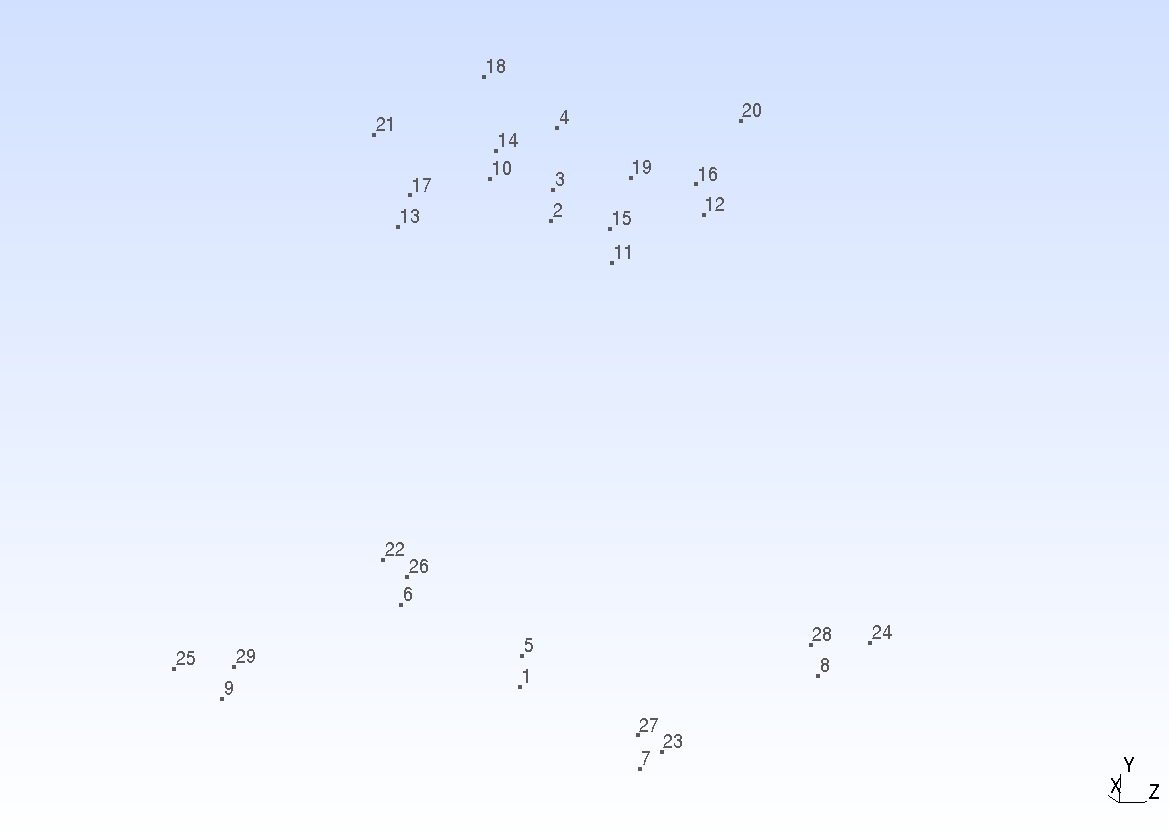
\includegraphics[scale=0.35]{pictures/main_points.png}
	\caption{Опорные точки}
	\label{fig: main_points}
\end{figure}

Для дальнейших построений (в наших масштабах) удобнее использовать
графический интерфейс \texttt{Gmsh}.

Соединим опорные точки так, чтобы получился наш каркас (рисунок \ref{fig: skeleton}).

\begin{figure}
	\center
	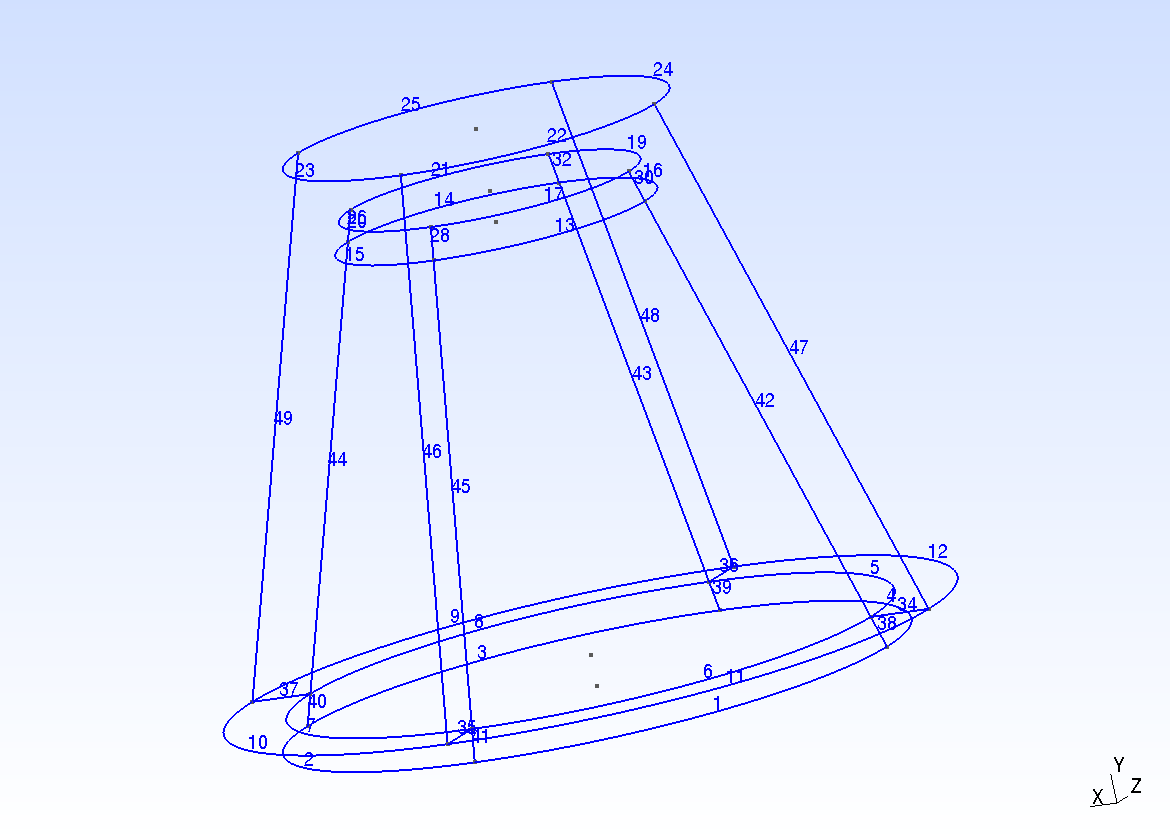
\includegraphics[scale=0.35]{pictures/skeleton.png}
	\caption{Каркас области}
	\label{fig: skeleton}
\end{figure}

\newpage
Далее, задавая контуры как замкнутые циклы линий,
 можно задать поверхности (рисунок \ref{fig: surfaces}).

\begin{figure}[H]
	\center
	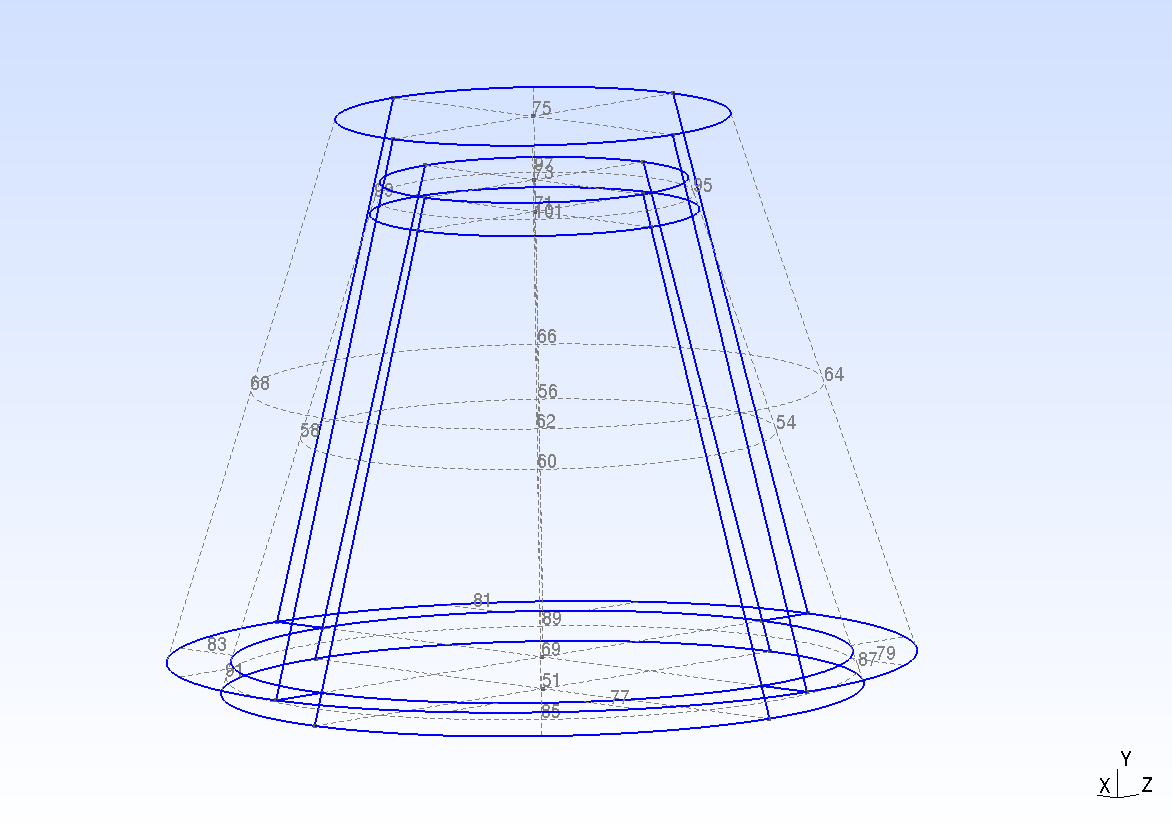
\includegraphics[scale=0.3]{pictures/surfaces.png}
	\caption{Поверхности}
	\label{fig: surfaces}
\end{figure}

Затем, путем объединения поверхностей в замкнутые объемы, можно 
задавать трехмерные области (рисунок \ref{fig: volumes}).

\begin{figure}[H]
	\center
	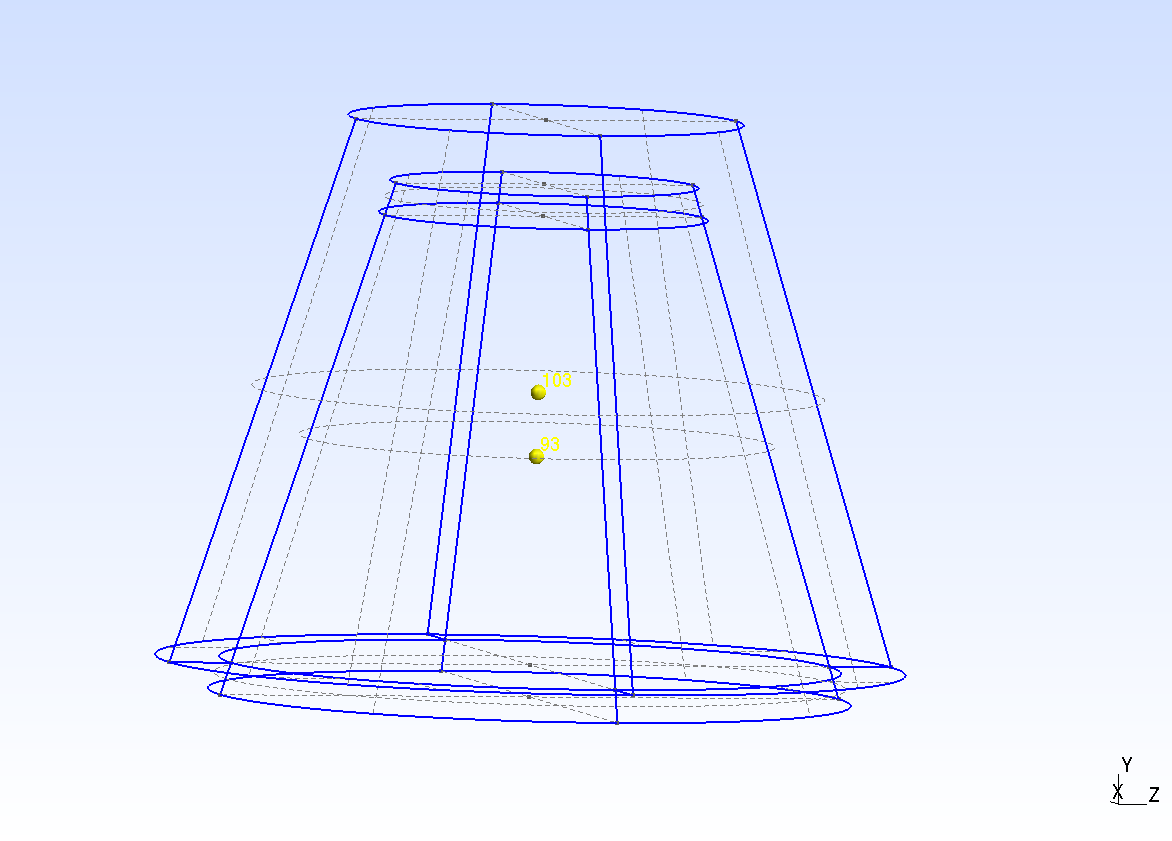
\includegraphics[scale=0.35]{pictures/volumes.png}
	\caption{Области}
	\label{fig: volumes}
\end{figure}

\subsection{Генерация сетки}

Итак, область построена, теперь нужно сгенерировать сетку.

\texttt{Gmsh} позволяет генерировать 1D, 2D, 3D сетки с помощью 
GUI либо консольных команд, имеет некоторые инструменты
для настройки построенной сетки, различные режимы ее отображения
и, разумеется, предоставляет возможность сохранять построенную сетку в файл.

На рисунке \ref{fig: mesh_display}
проиллюстрирована наша сетка в режиме отображения границ
поверхностей ячеек и в режиме отображения самих ячеек со срезом.

\begin{figure}[H]
	\begin{subfigure}[h]{0.5\textwidth}
		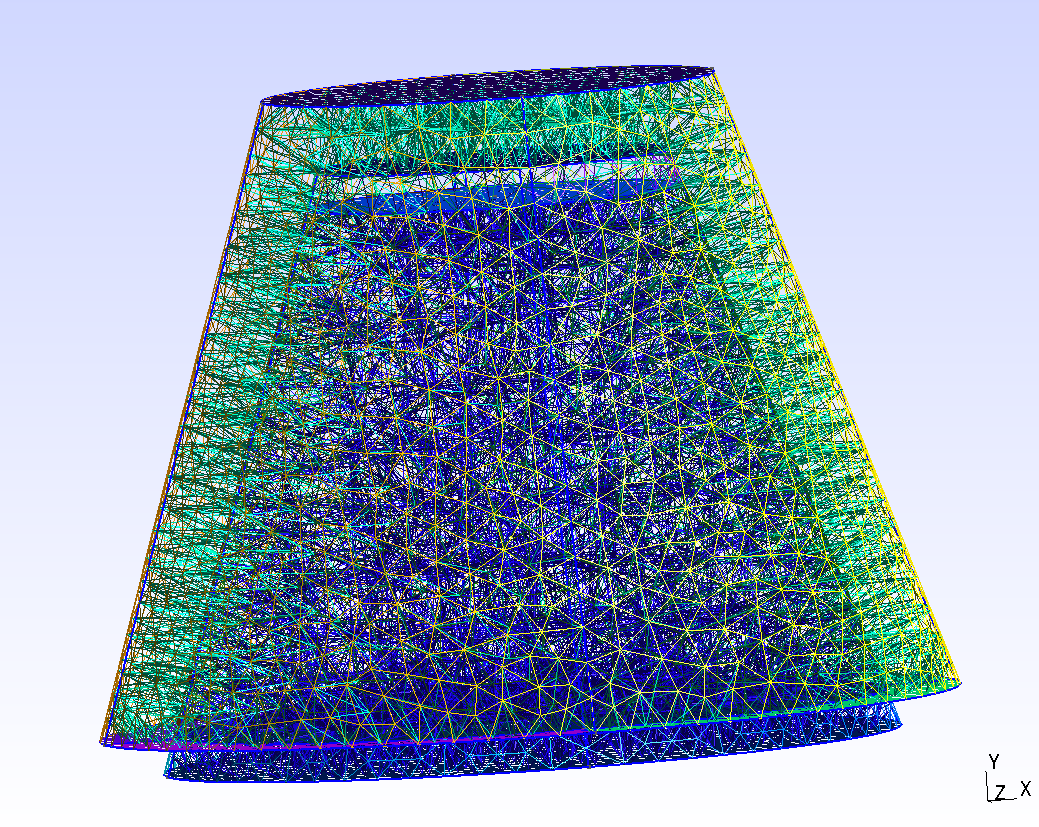
\includegraphics[scale=0.23]{pictures/mesh_surfaces_edges_full.png}
	\end{subfigure}
	\begin{subfigure}[h]{0.5\textwidth}
		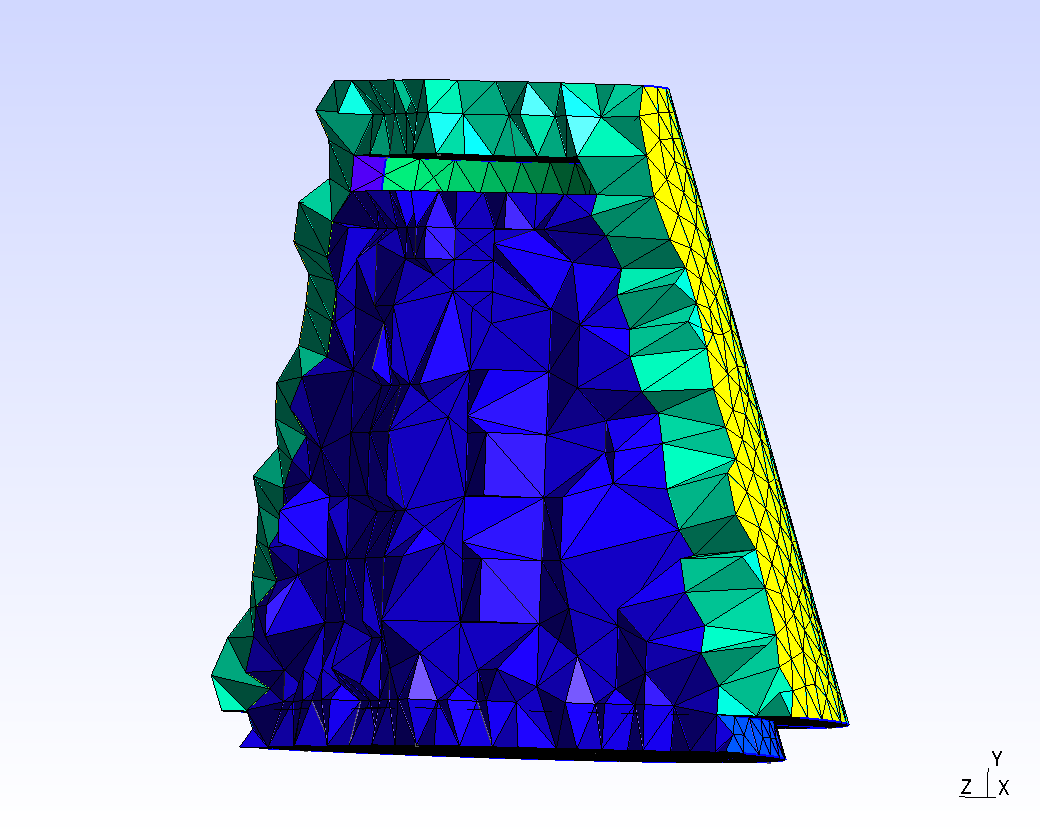
\includegraphics[scale=0.23]{pictures/mesh_volumes_slice.png}
	\end{subfigure}
	\caption{Примеры визуализации сетки (границы поверхностей элементов сетки и срез с отображением самих ячеек)}
	\label{fig: mesh_display}
\end{figure}

Для построения сетки и последующим преобразованием его к формату, который 
мы будем использовать в дальнейшем, используется следующий скрипт на языке \texttt{Python}:

\begin{lstlisting}
import os
os.system("gmsh -3 -format msh ./domain/final.geo")
os.system("dolfin-convert ./domain/final.msh ./domain/mesh.xml")
\end{lstlisting}

В итоге будем иметь несколько \textbf{.xml} файлов с описанием
сетки на нашей области.

\section{Описание численного алгоритма}

Для реализации численного алгоритма будем использовать open-source
инструмент \texttt{FEniCS} (\cite{fenics_book}), который предназначен для решения методом
конечных элементов задач, описываемых уравнениями в частных производных. 

Перейдем теперь к описанию решения нашей задачи.

Для начала прочитаем из файла параметров, собственно, параметры:
\begin{lstlisting}
param_file = File("problem.xml")
params = Parameters("parameters")
param_file >> params
info(params, True)
\end{lstlisting}

Достанем из параметров значения прилагаемой нагрузки и
коэффициенты Юнга и Пуассона, по которым вычислим коэффициенты Ламе:
\begin{lstlisting}
nu_values = np.array([params['coefficients']['Poisson'][
                     '1'], params['coefficients']['Poisson']['2']])
E_values = np.array([params['coefficients']['Young']['1'],
                     params['coefficients']['Young']['2']])
g_value = [params['boundCoefficients']['g']['1']['x'],
           params['boundCoefficients']['g']['1']['y'],
           params['boundCoefficients']['g']['1']['z']]
mu_values = E_values / (2.0 * (1.0 + nu_values))
lmbd_values = E_values * nu_values / \
    ((1.0 + nu_values) * (1.0 - 2.0 * nu_values))
\end{lstlisting}

Используемые значения коэффициентов Юнга и Пуассона характерны для
 материалов кости зуба и никель-хромовой стали.

Прочитаем сгенерированную сетку, а также отдельно ячейки каждой подобласти
и каждой части границы. Для поверхностей ячеек вычислим вектор нормали:
\begin{lstlisting}
mesh = Mesh(params['mesh']['path'])
subdomains = MeshFunction("size_t", mesh, params['mesh']['domains'])
boundaries = MeshFunction("size_t", mesh, params['mesh']['bounds'])
n = FacetNormal(mesh)
\end{lstlisting}

Далее зададим коэффициенты Ламе каждой из областей:
\begin{lstlisting}
V0 = FunctionSpace(mesh, 'DG', 0)
mu = Function(V0)
lmbda = Function(V0)

help = np.asarray(subdomains.array(), dtype=np.int32)
mu.vector()[:] = np.choose(help, mu_values)
lmbda.vector()[:] = np.choose(help, lmbd_values)
\end{lstlisting}

Зададим пространство используемых конечных элементов,
функции $\textbf{g}$ и $\textbf{u}_0$, а также триальную и тестовую
функции $\textbf{u}$ и $\textbf{v}$:
\begin{lstlisting}
V = VectorFunctionSpace(mesh, "CG", 1)
g = Expression((str(g_value[0]), str(g_value[1]), str(g_value[2])))
u_0 = Expression(("0.0", "0.0", "0.0"))
u = TrialFunction(V)
v = TestFunction(V)
\end{lstlisting}

Для границы $\Gamma_1$ зададим условия типа Дирихле:
\begin{lstlisting}
bc = DirichletBC(V, u_0, boundaries, 2)
\end{lstlisting}

Объявим области для интегрирования по области $\Omega$ и по границе
$\partial\Omega$:
\begin{lstlisting}
dx = Measure('dx', domain=mesh, subdomain_data=subdomains)
ds = Measure('ds', domain=mesh, subdomain_data=boundaries)
\end{lstlisting}

Зададим тензор напряжений как функцию и вычислим линейную и билинейную формы:
\begin{lstlisting}
def sigma(v, mu, lmb):
    return 2.0 * mu * sym(grad(v)) + lmb * tr(sym(grad(v))) * \
        Identity(v.cell().topological_dimension())
a = inner(sigma(u, mu, lmbda), sym(grad(v))) * dx(0) + \
    inner(sigma(u, mu, lmbda), sym(grad(v))) * dx(1)
L = inner(g, v) * ds(1)
\end{lstlisting}

Запустив функцию \texttt{solve()} для нашей задачи,
\begin{lstlisting}
u = Function(V)
solve(a == L, u, bc)

displ_file = File(params['results']['displacement'])
displ_file << u
\end{lstlisting}
мы найдем вектор упругих деформаций для каждой точки области.

Также вычислим и некоторые другие величины для деформированного тела:
\begin{itemize}
	\item Смещенную сетку:
\begin{lstlisting}
mesh.move(u)
newmesh_file = File("./results/mesh.pvd")
newmesh_file << mesh
\end{lstlisting}

	\item Напряжения:
\begin{lstlisting}
W = TensorFunctionSpace(mesh, "CG", 1)
stress = Function(W)
stress = project(sigma(u, mu, lmbda), W)

stress_file = File(params['results']['stress'])
stress_file << stress
\end{lstlisting}

	\item Нормальные и тангенциальные напряжения:
\begin{lstlisting}
s = sigma(u, mu, lmbda)

n = FacetNormal(mesh)
T = dot(-s, n)

Tn = inner(T, n) 
Tt = T - Tn*n  

scalar = FunctionSpace(mesh, "DG", 0)
vector = VectorFunctionSpace(mesh, "DG", 1)
v = TestFunction(scalar)
w = TestFunction(vector)

normal_stress = Function(scalar)
shear_stress = Function(vector)
Ln = (1/FacetArea(mesh))*v*Tn*ds
Lt = (1/FacetArea(mesh))*inner(w, Tt)*ds
assemble(Ln, tensor=normal_stress.vector())
assemble(Lt, tensor=shear_stress.vector())

normal_stress_file = File("./results/normal_stress.pvd")
normal_stress_file << normal_stress
shear_stress_file = File("./results/shear_stress.pvd")
shear_stress_file << shear_stress
\end{lstlisting}
\end{itemize}

Полный листинг кода приведен в приложении А.

\section{Визуализация результатов}
Для визуализации результатов будем использовать open-source инструмент
\texttt{ParaView}.

Для начала рассмотрим случай, когда вектор приложенной нагрузки направлен
вниз, т.е. происходит процесс давления (рисунки \ref{fig: result_push_displacement_slice} - 
\ref{fig: result_push_shear_stress_partial}).

\begin{figure}[H]
	\center
	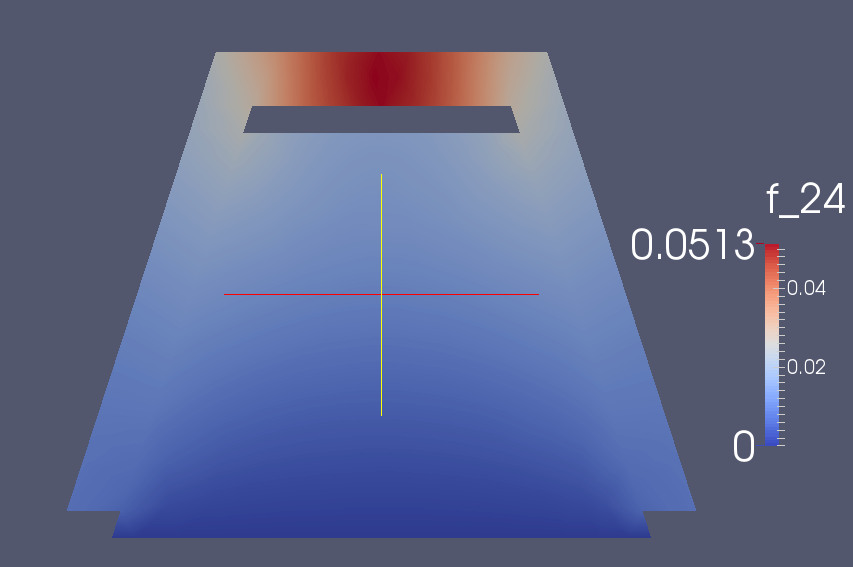
\includegraphics[scale=0.4]{pictures/result_push_displacement_slice.png}
	\caption{Модуль перемещений деформированного тела (разрез)}
	\label{fig: result_push_displacement_slice}
\end{figure}

\begin{figure}[H]
	\center
	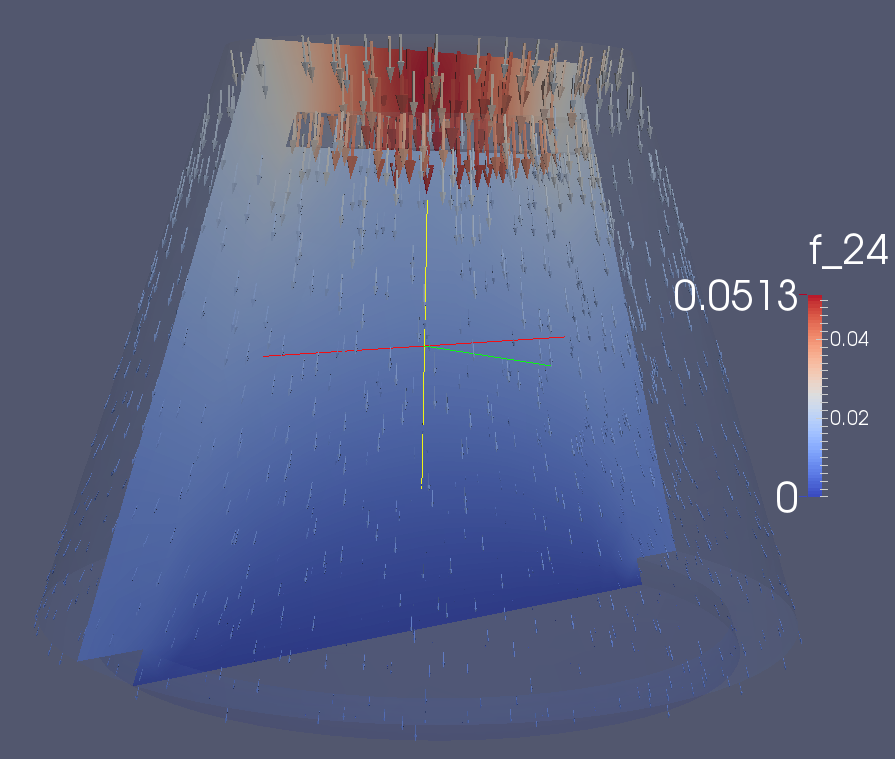
\includegraphics[scale=0.5]{pictures/result_push_displacement_glyph.png}
	\caption{Перемещения деформированного тела (glyph)}
	\label{fig: result_push_displacement_glyph}
\end{figure}

\begin{figure}[H]
	\center
	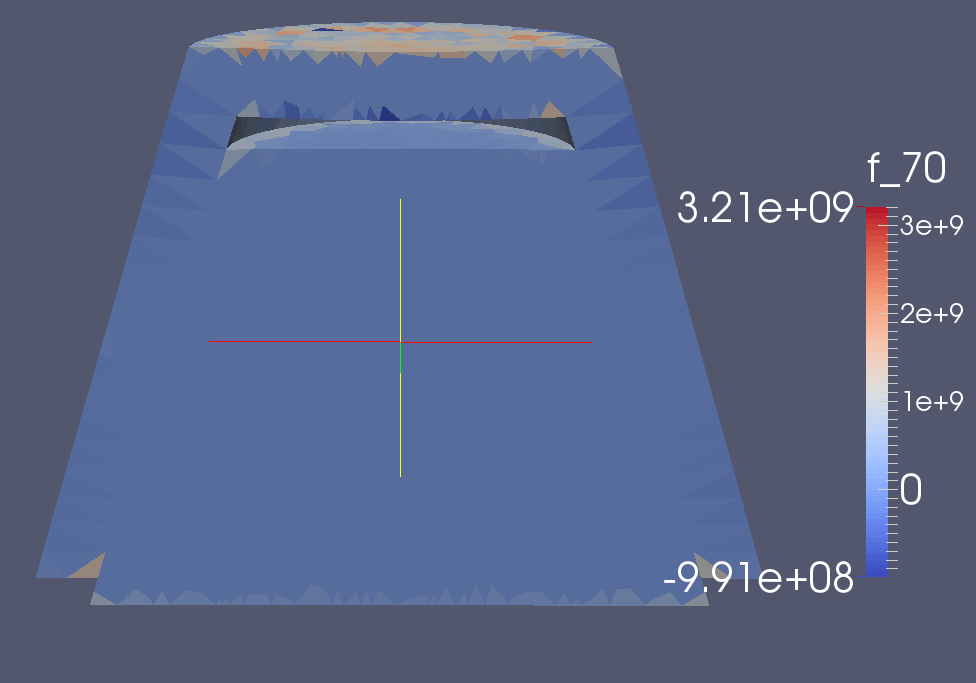
\includegraphics[scale=0.35]{pictures/result_push_normal_stress_slice.png}
	\caption{Нормальные напряжения деформированного тела}
	\label{fig: result_push_normal_stress_slice}
\end{figure}

\begin{figure}[H]
	\center
	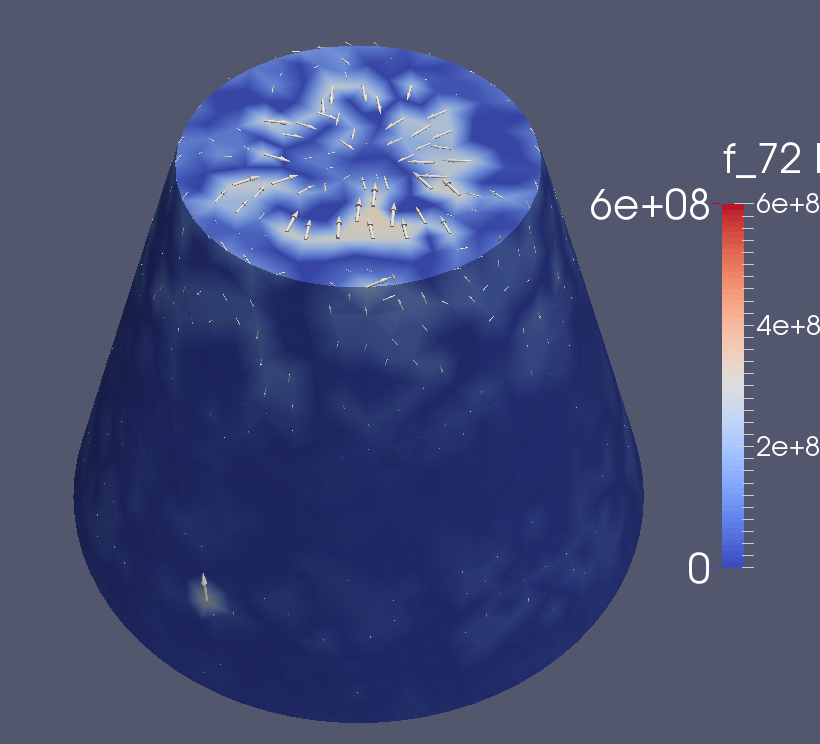
\includegraphics[scale=0.45]{pictures/result_push_shear_stress_full.png}
	\caption{Тангенциальные напряжения деформированного тела (внешняя поверхность)}
	\label{fig: result_push_shear_stress_full}
\end{figure}

\begin{figure}[H]
	\center
	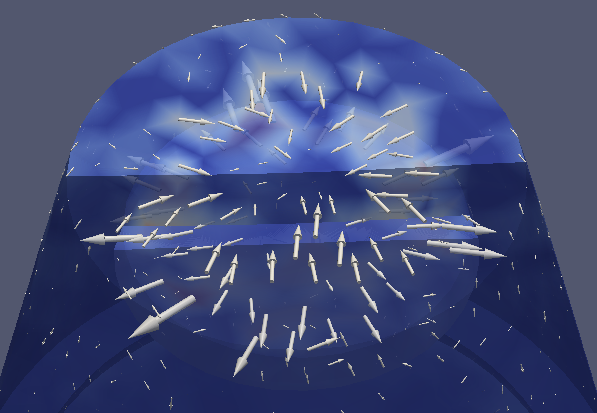
\includegraphics[scale=0.55]{pictures/result_push_shear_stress_partial.png}
	\caption{Тангенциальные напряжения деформированного тела (стыковочная часть)}
	\label{fig: result_push_shear_stress_partial}
\end{figure}

\newpage
Теперь рассмотрим случай, когда приложенная сила направлена вверх, т.е. коронку
пытаются стянуть (\ref{fig: result_pull_displacement_glyph} - \ref{fig: result_pull_shear_stress_partial}).

\begin{figure}[H]
	\center
	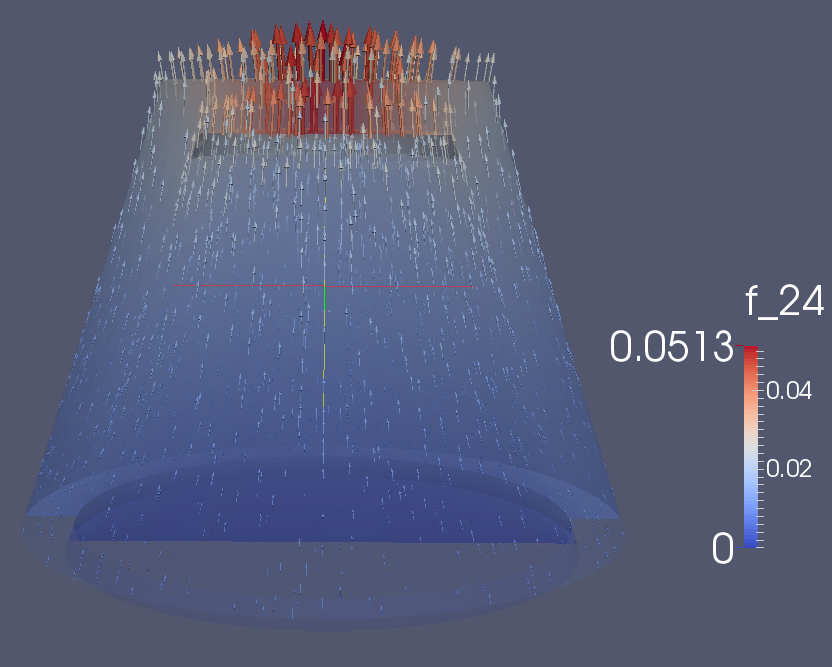
\includegraphics[scale=0.4]{pictures/result_pull_displacement_glyph.png}
	\caption{Перемещения деформированного тела (glyph)}
	\label{fig: result_pull_displacement_glyph}
\end{figure}

\begin{figure}[H]
	\center
	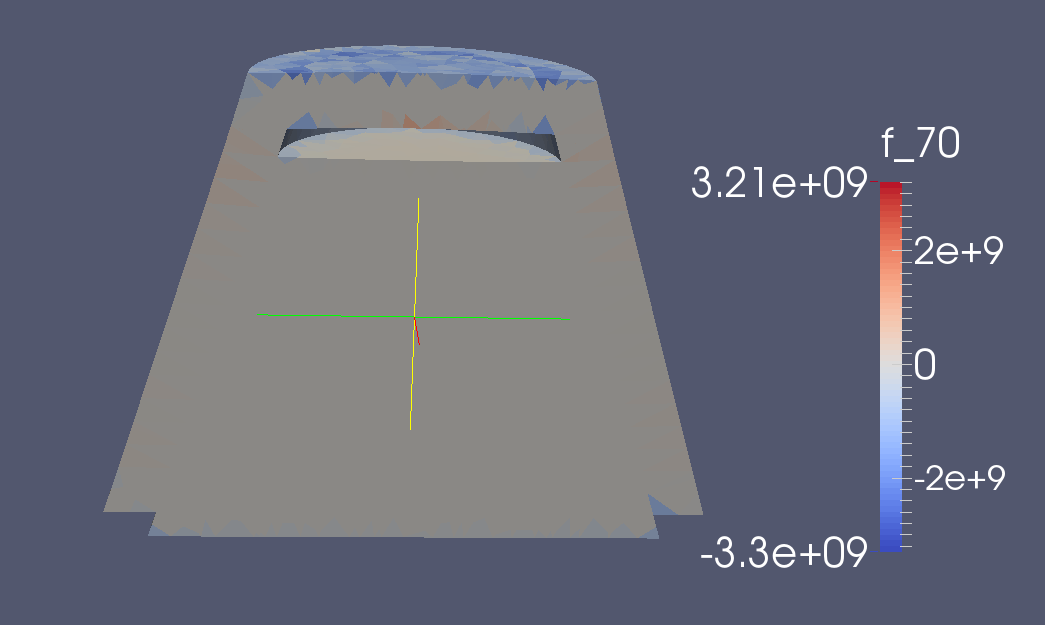
\includegraphics[scale=0.4]{pictures/result_pull_normal_stress_slice.png}
	\caption{Нормальные напряжения деформированного тела}
	\label{fig: result_pull_normal_stress_slice}
\end{figure}

\begin{figure}[H]
	\center
	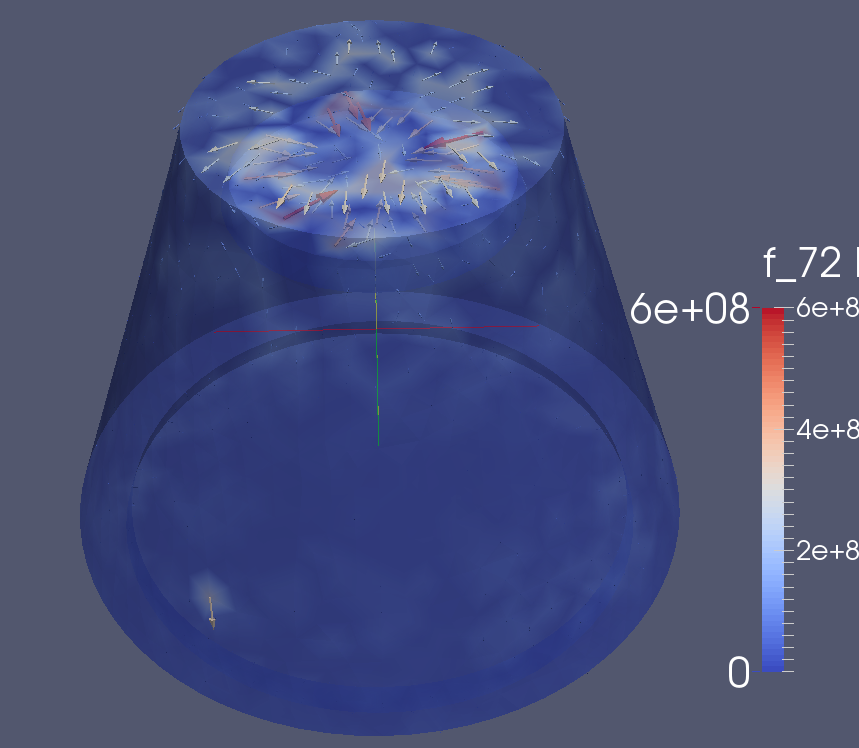
\includegraphics[scale=0.4]{pictures/result_pull_shear_stress_full.png}
	\caption{Тангенциальные напряжения деформированного тела (внешняя поверхность)}
	\label{fig: result_pull_shear_stress_full}
\end{figure}

\begin{figure}[H]
	\center
	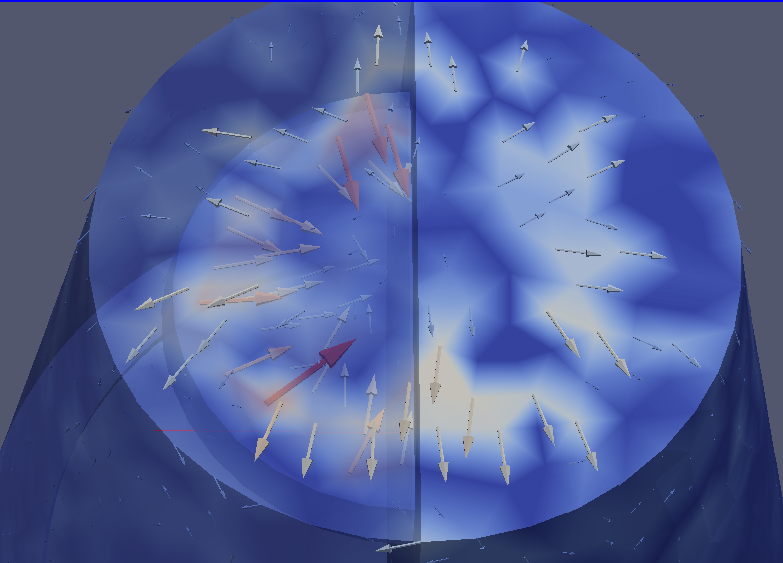
\includegraphics[scale=0.5]{pictures/result_pull_shear_stress_partial.png}
	\caption{Тангенциальные напряжения деформированного тела (стыковочная часть)}
	\label{fig: result_pull_shear_stress_partial}
\end{figure}

\newpage
\phantomsection
\begin{center}
\addcontentsline{toc}{section}{ЗАКЛЮЧЕНИЕ}
	\Large{\textbf{ЗАКЛЮЧЕНИЕ}}
\end{center}

В данной работе был рассмотрен пример краевой задачи теории
упругости в области сложной формы, был написан скрипт на языке \texttt{Python}
с использованием пакета \texttt{FEniCS}, который строит численное решение данной
задачи. 

Была проведена пара вычислительных экспериментов,
в ходе которых моделировались ситуации деформации нашей области
прикладываемыми нагрузками (давящая и тянущая силы), и провизуализированы
результаты вычислений.

В ходе работы использовались следующие инструменты:
\begin{itemize}
	\item Free-software пакет \texttt{Gmsh} для работы с областями
	различной формы и генерации на них сеток;
	\item Open-source пакет \texttt{FEniCS} для языка \texttt{Python},
	который предназначен для решения краевых задач методом конечных элементов;
	\item Open-source программа \texttt{ParaView} для иллюстрирования и
	визуального анализа результатов вычислений.
\end{itemize}




\newpage
\phantomsection
\renewcommand{\bibname}{\Large{СПИСОК ИСПОЛЬЗОВАННЫХ ИСТОЧНИКОВ}}
\addcontentsline{toc}{section}{СПИСОК ИСПОЛЬЗОВАННЫХ ИСТОЧНИКОВ}
\begin{thebibliography}{9}

	\bibitem{finite_element_method}
			Hughes Thomas J. R.,
			{The finite element method: linear static and dynamic finite element analysis} /
			Hughes Thomas J. R., -- Dover Publications, 2012. -- 704 c.
	\bibitem{math_elasticity_theory}
			Сьярле Ф.,
			{Математическая теория упругости} /
			Сьярле Ф. Перевод с англ. -- Г. А. Иосифьяна ; под ред. О. А. Олейник, -- Москва: Мир, 1992. -- 472 c.
	\bibitem{fenics_book}
			Logg A.,
			{Automated Solution of Differential Equations by the Finite Element Method. The FEniCS book} /
			Anders Logg, Kent-Andre Mardal, Garth N. Wells, -- Berlin: Shpringer, 2011. -- 720 c.
\end{thebibliography}



\newpage
	\phantomsection
\addcontentsline{toc}{section}{ПРИЛОЖЕНИЕ А}
\addcontentsline{toc}{section}{Листинг программы для решения задачи теории упругости}
\begin{center}
	\begin{flushright}
		\Large{\textbf{ПРИЛОЖЕНИЕ А}}\\
	\end{flushright}
	\textbf{Листинг программы для решения задачи теории упругости}
\end{center}

\lstinputlisting[basicstyle=\tiny, backgroundcolor = \color{white}, title=Data, language=XML]{../problem.xml}
\lstinputlisting[basicstyle=\tiny, backgroundcolor = \color{white}, title=Main]{../elasticity.py}
\lstinputlisting[basicstyle=\tiny, backgroundcolor = \color{white}, title=Mesh]{../meshgen.py}

\end{document}